\section{Neurobiología de la adicción}
Hasta hace algunos años persistían las ideas de que el abuso de sustancias era un acto voluntario y hedonista.
No obstante, la investigación de las últimas décadas ha venido apoyando la idea de que la adicción es una enfermedad del cerebro \parencite{Volkow2016}.\par
El modelo más reciente de la adicción la describe como un síndrome de inhibición de respuesta y atribución de saliencia dañada \parencite{Goldstein2012a}, compuesto por conductas impulsivas y compulsivas \parencite{Koob2010a} y caracterizado por:
\begin{enumerate}
    \item{compulsión en buscar y consumir la sustancia; }
    \item{pérdida de control limitando el consumo, y; }
    \item{emergencia de un estado emocional negativo reflejando un síndrome motivacional de abstinencia.}
\end{enumerate}
La adicción, entonces, en su estudio reciente suele dividirse en tres estados: intoxicación, abstinencia y afecto negativo, y, preocupación y anticipación (o \textit{craving}) \parencite{Koob2010a,Goldstein2012a,Volkow2016}.

\subsection{Intoxicación}
\label{intox}
Todas las drogas adictivas activan regiones cerebrales de recompensa en el cerebro que producen incrementos en la liberación de dopamina, lo que a su vez genera un aprendizaje asociativo o condicionamiento\footnote{En este tipo de aprendizaje Pavloviano, las experiencias recompensantes repetidas terminan asociándose con los estímulos mentales que les preceden.}.
Ante repetidas exposiciones, las neuronas dopaminérgicas dejan de disparar ante la droga en sí y responden de forma anticipatoria ante los estímulos condicionados. Esta liberación de dopamina desencadena neuroplasticidad\footnote{Cambios sistemáticos en la señalización o comunicación sináptica entre las neuronas.}; tanto como potenciación a largo plazo \textemdash donde la transmisión de señales entre las neuronas aumenta\textemdash{} como depresión a largo plazo \textemdash donde la señalización disminuye. Estos cambios en fuerza sináptica son controlados por la inserción o retiro de receptores glutamatérgicos (AMPA y NMDA) y cambios en la composición de sus subunidades \parencite{Volkow2016}. La regulación de los receptores AMPA incrementa la capacidad de respuesta del núcleo accumbens a glutamato libreado por terminales corticales y límbicas ante la exposición a drogas o estímulos relacionados \parencite{Wolf2010}. Cambios neuroplásticos han sido observados también en el estriado dorsal, la amígdala, el hipocampo y la corteza prefrontal \parencite{Volkow2016}.\par
Los estímulos ambientales relacionados al consumo, mediante este mecanismo, desencadenan una liberación rápida y condicionada de dopamina que provoca un antojo (o \textit{craving}) por la droga \parencite{Volkow2006}, motivan conductas relacionadas a la búsqueda de la sustancia y llevan a un uso compulsivo (atracón) \parencite{Volkow2016}.

\subsection{Abstinencia}
\label{abst}
Como resultado de los procesos fisiológicos condicionados, las recompensas ordinarias y saludables pierden su poder motivacional.
En las personas adictas se desarrolla un sesgo motivacional que provoca que los sistemas motivacionales y de recompensa se concentren en la liberación más potente de dopamina favorecida por la sustancia \textemdash{} y los estímulos ambientales condicionados al consumo de esta\parencite{Volkow2016}.\par
Contrario a lo que se podría pensar, estudios clínicos y pre-clínicos han demostrado que el consumo de sustancias produce incrementos mucho menores de los niveles de dopamina en la presencia de adicción en comparación con el consumo no dependiente \parencite{Volkow1997,Zhang2013,Volkow2014}.
Esta reducida liberación de dopamina deja al sistema de recompensa del cerebro mucho menos sensible a estímulos tanto relacionados, como no-relacionados a la sustancia; y como resultado, las personas con adicción no experimentan el mismo grado de euforia producida por el consumo al mismo tiempo que se sienten menos motivados por los estímulos de la vida diaria\footnote{Estos cambios no son inmediatamente reversibles e.g. desintoxicación.} \parencite{Volkow2016}.\par
Ante una exposición repetida a los efectos liberadores de dopamina de las sustancias ocurren adaptaciones en el circuito extendido de la amígdala, lo que resulta en un incremento en la reactividad ante el estrés y la emergencia de emociones negativas.
De esta forma, además de la motivación por la ``recompensa'' producida por el consumo, hay una motivación intensa a escapar de la disforia asociada con los efectos posteriores al uso \parencite{Goldstein2012a,Volkow2016}.\par
Este fenómeno está relacionado con la hipótesis de procesos-oponentes de \textcite{Solomon1978} que describe la dinámica temporal de respuestas emocionales opuestas.
Este modelo se puede observar cuando el refuerzo negativo (escapar de la disforia de la abstinencia) prevalece sobre el refuerzo positivo (la búsqueda del \textit{high} en la intoxicación aguda) en la transición del abuso ocasional de la sustancia al desarrollo de la adicción.\par
Desafortunadamente, aunque los efectos breves de incremento de dopamina posteriores al consumo alivian la aflicción de forma temporal, el resultado del consumo repetido es un incremento en la disforia durante la abstinencia, lo que lleva a un ciclo vicioso.

\subsection{Preocupación y anticipación}
\label{crav}
Los cambios que ocurren en los circuitos emocionales y de recompensa son acompañados por cambios en la función de regiones corticales prefrontales.
Entre los efectos de las alteraciones a estas regiones están la perturbación de procesos ejecutivos\footnote{Capacidades de auto-regulación, toma de decisiones, flexibilidad en la selección e inicio de la acción.}, la atribución de saliencia y el monitoreo del error \parencite{Goldstein2012a,Volkow2016}.
En sujetos con adicción, la señalización afectada de dopamina y glutamato en estas regiones prefrontales debilita la habilidad de resistir deseos fuertes o de seguir con la decisión de dejar el consumo de la sustancia \parencite{Volkow2016}.\par
El \textit{craving}, o el deseo fuerte e intenso de consumir la sustancia, tanto para volver a sentir los efectos eufóricos como para evitar los aspectos de abstinencia provocados por su ausencia, es un elemento clave en la recaída \parencite{Koob2010a}.
El \textit{craving} es entonces, por estas características, un punto clave como enfoque para el tratamiento de las adicciones.

\begin{figure}[!ht]
    \centering
    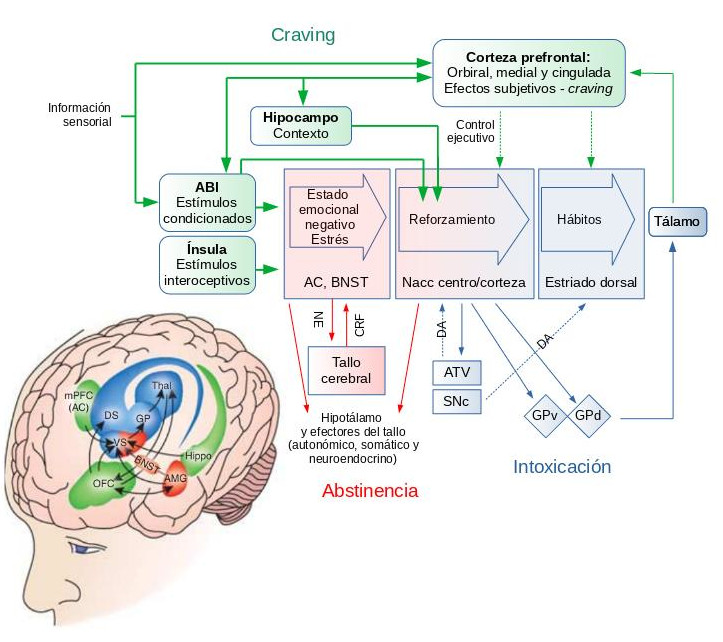
\includegraphics[width=0.9\textwidth]{reward.jpg}
    \caption{Esquema del circuito de recompensa involucrado en los procesos de adicción. Adaptado de \textcite{Koob2010a}. ABl, amígdala basolateral; AC, amígdala central; AMG, amígdala; ATC, área ventral tegmental; BNST, cama de la \textit{stria terminalis}; CRF, factor liberador de corticotropina; DA, dopamina; DS, estriado dorsal; Hippo, hipocampo; GP, globo pálido; GPd, globo pálido dorsal; GPv, globo pálido ventral; mPFC, corteza medial prefrontal; Nacc, núcleo accumbens; NE, norepinefrina; OFC, corteza orbitofrontal; SNc, \textit{substantia nigra pars compacta}; Thal, tálamo; VS, estriado ventral.}
    \label{fig:rew}
\end{figure}

\section{Tratamiento para la adicción a cocaína}
Actualmente no existe una cura para la adicción.
El tratamiento óptimo consiste en un abordaje multidisciplinario que ayuda al manejo de la enfermedad, compuesto generalmente por apoyo psicoterapéutico, consejería y tratamiento farmacológico en conjunto. \par
Este tratamiento no es de acceso universal. Una revisión del tratamiento de adicciones en México encontró que solo una pequeña proporción (16\%) de los usuarios de drogas acude alguna vez a tratamiento \parencite{Rojas2011}.\par
Y aun aquellos que sí buscan tratamiento, debido a la naturaleza crónica de la adicción, es muy probable que vuelvan a consumir \parencite{NIDA.}.
Estudios de seguimiento a 1 año postratamiento\footnote{Datos de tratamientos en EEUU.} han encontrado que solo el 40-60\% de los pacientes que pasan por una rehabilitación se mantienen en abstinencia \parencite{McLellan2000a}.\par
Debido a esto es de suma importancia la revisión del manejo actual de la adicción y la búsqueda de nuevos tratamientos alternativos que sean más efectivos.

\subsection{Tratamiento farmacológico}
No existe un tratamiento farmacológico aprobado por la FDA (\textit{Food and Drug Administration}; administración de alimentos y medicamentos, por sus siglas en inglés) de Estados Unidos para la dependencia a la cocaína.
Los medicamentos utilizados son los mismos que aquellos usados para tratar la epilepsia o los espasmos musculares; con el fin de aliviar la ansiedad y la agitación resultantes de la adicción a la cocaína.
Algunos de estos son: gabapentina, un anticonvulsivante análogo a GABA; modafinilo, promotor del estado de alerta inhibiendo la re-captura de dopamina; topiramato, anticonvulsivante que alivia la agitación; vigabatrina, anti-epiléptico usado para el \textit{craving} inhibiendo el catabolismo de GABA; y, baclofeno, relajante muscular agonista de GABA \parencite{Volkow2007b}.\par
De todos los medicamentos usados para tratar la adicción a la cocaína, disulfiram es el que ha tenido más resultados exitosos consistentes \parencite{Volkow2007b}.
Usualmente utilizado como tratamiento para la adicción al alcohol por medio de la inducción de una reacción adversa a su consumo, el disulfiram también ha sido prescrito para desalentar el uso de la cocaína.
Aún se desconoce su funcionamiento específico en el tratamiento de la dependencia a la cocaína, pero sus efectos pueden estar relacionados a su capacidad de inhibir una enzima que convierte a la dopamina en noradrenalina.
Sin embargo, no es efectivo para todas las personas, ya que se ha visto que ciertas variaciones genéticas influyen en la efectividad del tratamiento \parencite{Gaval-Cruz2009a, Volkow2007b}.

\subsection{Tratamiento comportamental}
Junto al tratamiento farmacológico, se lleva a cabo un abordaje comportamental por medio de psicoterapia y consejería.
Entre los modelos más utilizados \parencite{Volkow2008} dentro de estas áreas están:
la psicoterapia cognitivo-conductual, donde el paciente aprende a identificar y corregir comportamientos problemáticos aplicando una serie de técnicas que pueden ser usadas para detener el abuso de la sustancia y abordar los problemas que suelen ocurrir en conjunto;
el manejo de contingencias, en el cual, por medio de recompensas tangibles se refuerzan los comportamientos deseados como el dejar de consumir la sustancia;
intervención motivacional, un abordaje de consejería donde se ayuda al paciente a resolver su ambivalencia sobre el compromiso al tratamiento y parar el consumo de la sustancia;
y la terapia familiar conductual, que intenta abordar no solo el consumo de la droga, sino también los problemas en conjunto, como trastornos de conducta, maltrato infantil, depresión, conflictos familiares y desempleo.

\section{Estimulación magnética transcraneal repetitiva}
A pesar de ser desarrollada como una herramienta diagnóstica para trastornos motores, la estimulación magnética transcraneal (EMT) puede modular, transitoria o duraderamente la excitabilidad cortical por medio de la aplicación de pulsos electromagnéticos localizados que pasan de forma indolora y sin daño por la piel y el cráneo \parencite{Horvath2011a, Noohi2016}.
La EMT puede ser aplicada por medio de pulsos individuales, pulsos pareados, por medio de repetidos trenes de estimulación, continuos o a una frecuencia específica (repetitiva o EMTr) o bajo un patrón de intervalos inter-tren específico (estimulación \textit{theta-burst} continua, ETBc; o intermitente, ETBi) \parencite{Ekhtiari2019}. \par
Se ha observado que la EMTr a alta frecuencia (\deactivatequoting\SI{> 5}{\hertz}\activatequoting) facilita la excitabilidad cortical-motora, mientras que a baja frecuencia (\deactivatequoting\SI{< 1}{\hertz}\activatequoting) la inhibe \parencite{Pascual-Leone1994}.
De la misma forma, la estimulación con \textit{theta-burst} (ETB) presenta patrones similares de estimulación e inhibición cortical en sus modalidades intermitente y continua respectivamente, pero con una duración menor que la EMTr. El mecanismo primario hipotetizado bajo los efectos neuromoduladores de ambas técnicas es la potencialización a largo plazo (LTP) y depresión a largo plazo (LTD).
Un rápido incremento postsináptico de iones de calcio puede inducir LTP, lo que se ha observado en EMTr de alta frecuencia (\SI{10}{\hertz}) y en ETBi; mientras que un flujo mas lento y sostenido de calcio induce LTD en EMTr de (\SI{1}{\hertz}) y ETBc \parencite{Ekhtiari2019}.

\subsection{EMTr como tratamiento para la adicción}
Las investigaciones recientes apoyan el uso de la EMTr de reducir el \textit{craving} de tabaco, alcohol y cocaína en pacientes con adicción \parencite{Barr2011}.
La mayoría de los estudios clínicos en adicción se enfocan en estimular la corteza dorsolateral prefrontal izquierda \parencite{Bellamoli2014a,Barr2011,Ekhtiari2019}.
Varias líneas de evidencia sugieren que la estimulación sobre esta región puede influir en las regiones cerebrales involucradas en la adicción:
\begin{enumerate}
    \item La corteza prefrontal dorsolateral está conectada al sistema dopaminérgico meso-fronto-límbico, el sistema cerebral de recompensa asociado al \textit{craving} \parencite{Barr2011}.
    \item Se ha demostrado la capacidad de la EMTr de inducir liberación de dopamina en áreas corticales y subcorticales \parencite{Cho2009,Strafella2001}, lo que podría mitigar la disfunción dopaminérgica asociada a la adicción.
    \item El nivel de \textit{craving} a comida, alcohol y tabaco en la presencia de estímulos visuales se ha reducido con la estimulación de la corteza prefrontal dorsolateral con EMTr \parencite{Amiaz2009}.
    \item Se ha encontrado que la corteza prefrontal dorsolateral está involucrada con procesos de toma de decisiones; los cuales pueden estar alterados en pacientes con adicción, quienes tienen mayor probabilidad a ser impulsivos y tener comportamientos asociados a la toma de riesgos \parencite{Barr2011}.
\end{enumerate}
Las características neuromoduladoras y los cambios plásticos observados como efecto de la EMTr hacen de esta un tratamiento factible para alterar los circuitos involucrados en el \textit{craving}, lo que, por efecto, llevaría a la disminución de la recaída y una mayor efectividad de tratamiento.

\subsubsection{EMTr y adicción a cocaína}
El consumo crónico de cocaína está asociado con una disrupción en la conectividad fronto-estriatal en estado de reposo; una elevada actividad en la corteza prefrontal medial y estriado ventral, y una actividad deprimida en la corteza prefrontal dorsolateral y estriado dorsal, así como una disminución en la transmisión dopaminérgica mesolímbica, lo que mantiene el consumo de la droga \parencite{Rachid2018}.
Estas afectaciones tienen un rol importante en el desarrollo de la adicción, lo que se amplifica y soporta por una incontrolable necesidad de consumir la substancia (\textit{craving}), lo que conduce a su búsqueda y relapso.
En efecto, se ha encontrado que mayores índices de \textit{craving} se relacionan con índices más altos de recaída \parencite{Sinha2006,Volkow2000a,Volkow2016}.
Por esto mismo, investigaciones recientes han buscado explorar los efectos terapéuticos de la estimulación de la corteza prefrontal por medio de EMTr en la adicción a cocaína \parencite{Bolloni2018}. \par
\textcite{Camprodon2007} fueron los primeros en explorar los efectos de la EMTr en el \textit{craving} de cocaína.
Encontraron un efecto transitorio en el \textit{craving} de cocaína después de una sesión de EMTr sobre la corteza prefrontal dorsolateral derecha \textemdash{}pero no la izquierda.
Desde entonces, diversos estudios han encontrado que la EMTr sobre la corteza prefrontal izquierda es capaz de reducir el \textit{craving} \par
\textcite{Politi2008} observaron que después de 10 sesiones de EMTr a \SI{15}{\hertz} había una disminución del \textit{craving} en 36 sujetos con dependencia a cocaína, encontrando un efecto después de la 7ma sesión.
\textcite{Terraneo2016}, en su estudio aleatorio abierto, compararon los efectos terapéuticos sobre la adicción a cocaína entre ocho sesiones de EMTr a \SI{15}{\hertz} (sesiones diarias por cinco días y una sesión semanal de mantenimiento por tres semanas) y un tratamiento farmacológico habitual.
Encontraron que había una mayor disminución del \textit{craving} en los sujetos del grupo de EMTr comparados con el grupo control, así como una diferencia significativa en la cantidad de pacientes que tuvieron un relapso\footnote{El consumo fue medido por medio de pruebas objetivas de orina}. \par
Aunque la mayoría de las investigaciones de EMTr en adicción se enfocan en la corteza prefrontal dorsolateral, estudios recientes han explorado los efectos sobre la estimulación de la corteza prefrontal ventromedial \parencite{Hanlon2015,Kearney-Ramos2018a}, argumentando que la corteza prefrontal medial es un método más directo de modular la actividad del núcleo accumbens\footnote{Las cortezas prefrontales orbital y medial son la principal entrada cortical al estriado ventral, que incluye al caudado y núcleo accumbens.}.
En un estudio piloto experimental, \textcite{Hanlon2015} obtuvieron datos de neuroimagen y de \textit{craving} antes y después de ETB continua sobre la corteza medial prefrontal izquierda y encontraron que una sesión de ETB real reducía el \textit{craving} comparado con la sesión placebo, así como una reducción de actividad sobre la corteza prefrontal y el núcleo accumbens.
\textcite{Kearney-Ramos2018a} exploraron los efectos de la ETB continua en la reactividad a estímulos relacionados a la sustancia y encontraron un efecto general de la ETBc atenuando el \textit{craving} después de la sesión real en comparación con la placebo, en usuarios de cocaína. \par
Otro enfoque de tratamiento utilizado en la EMTr es el empleo de la bobina H1 que permite la estimulación bilateral de regiones más profundas.
\textcite{Bolloni2016} observaron una disminución significativa en el consumo de cocaína en sujetos con adicción a cocaína a los tres y seis meses posteriores a un tratamiento real de EMTr profunda de 12 sesiones (tres a la semana) a \SI{10}{\hertz} sobre la corteza prefrontal bilateral\footnote{La interacción primaria (Tratamiento X Tiempo) fue no significativa en el análisis primario.} que no se encontró en el grupo placebo.\par
Por su parte, el equipo de \textcite{Rapinesi2016} utilizando la misma técnica de EMTr profunda (pero con una frecuencia mayor, tres sesiones semanales a \SI{15}{\hertz} por cuatro semanas) observaron una disminución significativa de \textit{craving} en sujetos con dependencia a la cocaína dos, cuatro y ocho semanas después del tratamiento.
No obstante, hubo un empeoramiento en los niveles de \textit{craving} después de la cuarta semana, aunque estos se mantuvieron por debajo de los niveles basales.

\section{Imagenología por resonancia magnética}
Aunque la imagenología radioisotópica (PET) ha sido muy significativa en el descubrimiento y mapeo del rol de la dopamina en la adicción, la imagenología por resonancia magnética (MRI) es el pilar de la investigación con neuroimagen en la adicción, debido a su seguridad, ausencia de radioactividad y flexibilidad en la información obtenida \parencite{Suckling2017}. \par
La MRI puede ofrecer información tanto anatómica \textemdash{}relacionada a la estructura de la materia gris y blanca\textemdash{} como funcional \textemdash{}relacionada a la actividad cerebral.

\subsection{Resonancia magnética funcional}
La resonancia magnética funcional (fMRI) es una técnica de neuroimagen que mide la actividad cerebral por medio del contraste endógeno del nivel dependiente de oxigenación de sangre (BOLD) \parencite{Ogawa1993} utilizando las distintas propiedades magnéticas de la sangre oxigenada y desoxigenada.
Partiendo de que la actividad neuronal requiere oxígeno, la señal BOLD está relacionada de forma indirecta con el procesamiento funcional local.
Los experimentos de fMRI, entonces, con frecuencia inducen procesos cognitivos específicos con los estímulos apropiados con la intención de observar las regiones y circuitos involucrados. \par
Mucho de lo que se conoce sobre función cerebral ha venido de estudios que miden los cambios en actividad neuronal y conducta después de la administración de una tarea o estímulo (\textit{task-based fMRI}, o fMRI de tarea), sin embargo, cambios espontáneos de la señal BOLD que no son atribuidos a un diseño experimental también están presentes \parencite{Fox2007}.
Es así como la resonancia magnética funcional en estado de reposo (\textit{resting-state fMRI}, o fMRI en reposo) ha emergido como una poderosa herramienta que permite medir la conectividad funcional \parencite{Biswal2010}.\par
La resonancia funcional durante el reposo revela fluctuaciones espontáneas de gran amplitud y baja frecuencia (\deactivatequoting\SI{< 0.1}{\hertz}\activatequoting) que pueden ser temporalmente correlacionadas entre áreas relacionadas funcionalmente.
Un único escaneo (de al menos cinco minutos) puede ser usado para estudiar una multitud de circuitos funcionales \parencite{Biswal2010}.

\subsection{Resonancia magnética funcional en adicción}
Las investigaciones de neuroimagen sobre la neurobiología de las adicciones han sido en su mayoría realizadas por técnicas como la tomografía por emisión de positrones (PET) o la fMRI por medio de tareas, las cuales tienen que ver con la presentación de señales o impulsos relacionados con la sustancia \parencite{Jasinska2014}.
Como se mencionó en la sección \ref{intox}, es común en muchos de los comportamientos adictivos la reacción ante estímulos relacionados con el consumo y consecuentemente la inducción de \textit{craving} como consecuencia de un condicionamiento Pavloviano.\par
Al revisar la literatura, \textcite{Suckling2017} encontraron que en los sujetos con adicción hay un incremento en la activación en regiones prefrontales y orbitofrontales y que las regiones con una reactividad a estímulos relacionados al consumo convergían a la corteza del cíngulo anterior, amígdala y estriado ventral en sujetos con adicción a la nicotina, alcohol y cocaína. \par
El control inhibitorio es la supresión de acciones prepotentes y la resistencia a interferencia de estímulos externos para emplear comportamientos dirigidos a metas.
En individuos con adicción a cocaína se observó una actividad incrementada en las cortezas del cíngulo y prefrontal, regiones frontales inferiores y cerebelo durante la inhibición de respuesta, independientemente de si la acción fue inhibida con éxito o no \parencite{Suckling2017}.\par
En una tarea \textit{go/no-go}, sujetos con adicción a cocaína mostraron mayor cantidad de errores por omisión y comisión que controles, lo que se atribuyó a una hipoactivación de la corteza dorsal anterior del cíngulo en los ensayos \textit{stop} \parencite{Kaufman2003}.
En un segundo estudio se encontró que este déficit inhibitorio en usuarios de cocaína era agravado por una mayor carga de memoria de trabajo, y de nuevo, una activación de la corteza dorsal anterior del cíngulo fue relacionada con el déficit conductual \parencite{Hester2004}.\par
Otro estudio que investigaba cómo los sujetos con adicción a cocaína y controles respondían ante recompensas monetarias por un correcto desempeño en una tarea de atención encontró que aquellos sujetos con adicción a cocaína mostraban señales BOLD reducidas en la corteza orbitofrontal izquierda en ganancias altas comparados con controles además de ser menos sensibles a la diferencia del valor de las recompensas en la actividad de la corteza orbitofrontal y la corteza prefrontal dorsolateral \parencite{Goldstein2007}. \par
\textcite{Connolly2012} exploraron los diferentes patrones de control cognitivo en sujetos con dependencia a cocaína con diferente tiempo de abstinencia y controles;
entre sus hallazgos encontraron que todos los grupos mostraban un nivel de desempeño similar, los sujetos con adicción tenían una mayor activación asociada con el control inhibitorio y el monitoreo de desempeño. Pero más importante, los dos grupos de sujetos con dependencia mostraron diferencias entre sí en los niveles de activación, sugiriendo diferentes demandas de control cognitivo relacionadas a la duración de abstinencia: el grupo de abstinencia corta tenía una activación en regiones dorsales de los giros frontales medio y superior, mientras que los de abstinencia mayor tendían a reclutar áreas más inferiores, como el giro frontal inferior bilateral.
De igual forma, ambos grupos de adictos presentaron regiones de actividad cerebelares en contraste con los controles, lo que podría sugerir que como usuarios activos de la sustancia tienden a depender de estas regiones como una compensación de la atrofia prefrontal, lo que se mantiene en la abstinencia. \par
Diversos estudios que incorporan el procesamiento emocional con tareas cognitivas indican que la corteza prefrontal dorsolateral es principalmente hiperactiva durante el procesamiento de emociones en individuos con adicción comparado con controles; especialmente en emociones negativas; la corteza cingular anterior ha mostrado resultados mixtos \textemdash{}con más estudios mostrando hipoactividad que hiperactividad\footnote{Es posible que la hiperactividad de la corteza prefrontal dorsolateral esté compensando la hipoactividad de la corteza del cíngulo anterior.} \parencite{Goldstein2012a}.\par
Tareas que involucran respuestas emocionales activan el sistema límbico. En un estudio que buscaba observar las diferencias en el procesamiento emocional entre sujetos con adicción y controles encontró que había una diferencia inter-grupal significativa en las regiones de procesamiento emocional \parencite{Asensio2010}; el grupo de adicción a cocaína mostró una menor activación en el estriado derecho, tálamo izquierdo, corteza prefrontal dorsolateral y giro parietal con las imágenes placenteras y una hiperactivación del giro parietal superior y corteza prefrontal dorsomedial ante las imágenes placenteras, mostrando una disregulación de valencia en los mecanismos de procesamiento de emociones.
La hipoactivación de la corteza dorsomedial ante estímulos placenteros sugiere una dañada evaluación ante recompensas y disminuida atribución de saliencia y motivacional hacia estímulos placenteros, mientras que la hipoactivación estriatal y dorsolateral prefrontal puede ser la causante de la habilidad reducida de experimentar placer de los estímulos reforzadores naturales (ver sección \ref{abst}).

\subsection{Resonancia magnética funcional en reposo en adicción}
Son pocos los estudios de conectividad funcional en estado de reposo en el campo de las adicciones, especialmente comparados con los que utilizan las técnicas anteriores.
Relacionado al abuso de la heroína, se ha encontrado alteraciones en la conectividad funcional entre regiones límbicas \textemdash{}como el núcleo accumbens, amígdala, núcleo caudado\textemdash{} y regiones frontales \textemdash{}como la corteza orbitofrontal y el cíngulo \parencite{Ma2010,Tianye2015,Wang2010,Zhang2016}.\par
En pacientes con adicción a la cocaína se ha observado una disminución en la conectividad del sistema meso-cortico-límbico; entre el área tegmental ventral y el núcleo accumbens, y el tálamo; entre la amígdala y la corteza prefrontal medial; así como entre el hipotálamo y la corteza prefrontal medio-dorsal.
Esta disminución en conectividad estaba negativamente relacionada con el tiempo de adicción \parencite{Gu2010}.
De igual forma, se ha encontrado una correlación negativa entre el \textit{craving} subjetivo y la actividad del giro medial-posterior del cíngulo en adictos a la cocaína.
En el mismo estudio se observó una relación entre las áreas que procesan las señales relacionadas a la droga (corteza orbitofrontal y estriado ventral);
así como una conectividad negativa entre estas áreas y el giro medial posterior del cíngulo \parencite{Wilcox2011}.\par
Se han reportado diferencias interhemisféricas en las regiones frontales entre consumidores y sujetos control;
así como una reducción en la conectividad funcional interhemisférica entre nodos de la red de atención dorsal (áreas latero-frontales bilaterales, premotoras mediales y parietales posteriores), lo que podría sugerir que estas anormalidades se relacionan a los problemas de atención presentados en la adicción \parencite{Kelly2011a}.
\textcite{Verdejo-Garcia2014} hallaron menor conectividad funcional entre corteza anterior del cíngulo, tálamo, ínsula y tallo cerebral; así como alteraciones funcionales en los sistemas fronto-límbicos.\par
\textcite{Hu2015} encontraron una conectividad aumentada en los circuitos fronto-estriatales de los usuarios de cocaína, los cuales también presentaron una conexión reducida entre el estriado y las regiones del cíngulo, estriado, hipocampo/amígdala e ínsula. El uso compulsivo de la cocaína fue asociado con un balance entre un aumento de la conectividad anteroestriatal-prefrontal/orbital y una disminución de la conectividad estrato-dorsal anterior del cíngulo.\par
Los primeros estudios de conectividad efectiva en usuarios de cocaína en abstinencia encontraron una mayor conectividad del área tegmental ventral a: núcleo accumbens, hipocampo y corteza frontal-medial; así como una menor conectividad de la corteza frontal-medial a el área tegmental ventral y del núcleo accumbens a corteza frontal-medial  \parencite{Ray2017,Ray2016}.\par
Estos estudios de neuroimagen y conectividad permiten tener una visión de los circuitos involucrados en la adicción, así como un marco de referencia para evaluar el cambio producido por el tratamiento.

\section{Análisis de redes complejas}
Desde el siglo XIX es bien sabido que los elementos neuronales constituyen una formidable y complicada red estructural.
A partir de los años 1990s, el aumento de nuestro entendimiento de la física de los sistemas complejos ha llevado al desarrollo de la \emph{ciencia de las redes}, un esfuerzo interdisciplinario de caracterizar las propiedades importantes de los sistemas complejos por medio de la cuantificación de las topologías de sus respectivas representaciones en redes \parencite{Bullmore2009a,Rubinov2010}.\par
Este análisis de redes complejas tiene su origen en el estudio matemático de redes conocido como \emph{teoría de grafos}, con la diferencia que este análisis tiene como objeto de estudio redes de la vida real que son grandes y complejas y no uniformemente ordenadas ni aleatorias \parencite{Rubinov2010}.\par
Los datos de conectividad cerebral pueden estudiarse como redes de regiones cerebrales conectadas por tractos anatómicos o asociaciones funcionales;
son indudablemente complejas, comparten características con otras redes biológicas y sistemas físicos y, por lo tanto, pueden ser categorizadas usando métodos de redes complejas.
Estos análisis permiten cuantificar con confiabilidad las redes cerebrales con un pequeño número de medidas fácilmente computables y neurobiológicamente significativas \parencite{Humphries2008,Latora2001,Achard2007}. \par

Una red es una representación matemática de un sistema complejo del mundo real; es definida por una colección de nodos y conexiones (o aristas) entre pares de nodos \parencite{Bullmore2009a,Rubinov2010}. \par
Las redes estructurales o funcionales del cerebro pueden ser estudiadas por medio de la metodología de redes complejas siguiendo los siguientes pasos:
\begin{enumerate}
    \item Definir los nodos de la red.
        Estos pueden ser definidos como los electrodos en un estudio de electroencefalograma o regiones anatómicamente definidas de datos de MRI.
        Idealmente deberían representar regiones cerebrales con patrones coherentes de conexiones anatómicas o funcionales.
        Las parcelaciones utilizadas deben cubrir completamente la superficie de la corteza o el cerebro entero y nodos individuales no deben traslaparse espacialmente.
    \item Calcular las aristas estimando una medida continua de asociación entre los nodos.
        Esta medida puede tener bases funcionales, como el coeficiente de correlación entre las fluctuaciones de la señal BOLD en una corrida de fMRI, o anatómicas, como la probabilidad de la presencia de tractos de sustancia blanca calculada por medio de MRI de difusión.
    \item Aplicar un umbral.
        Aristas débiles o no significativas pueden representar conexiones espurias.
        Estas aristas tienden a opacar la topología de conexiones fuertes y significativas por lo que generalmente son descartadas por medio de un umbral absoluto o proporcional.
        Las aristas resultantes pueden ser binarias, representando únicamente la presencia (1) o ausencia de la conexión (0), o ponderadas, si además incluyen información adicional sobre la magnitud de la conexión.
    \item Generar una matriz de asociación compilando todas las asociaciones entre pares de los nodos.
        Todas las auto-conexiones o conexiones negativas (en el caso de representaciones gráficas de fMRI, anti-correlaciones de la señal BOLD) deben ser removidas de las redes antes del análisis \parencite{Rubinov2010}.
    \item Calcular y analizar la topología de la red.
        Una vez calculados los parámetros de redes de interés en este modelo gráfico de red cerebral, se comparan entre grupos o contra parámetros equivalentes en una población de redes aleatorias.
\end{enumerate}

\subsection{Métricas de topología de red}
En teoría de grafos $N$ es el conjunto de todos los nodos de una red y $n$ el número de nodos.
Del mismo modo, $L$ es el conjunto de aristas en la red y $l$ el número de aristas.
$(i,j)$ es la conexión o arista entre los nodos $i$ y $j$, $(i,j \in N)$.
$a_{ij}$ es el estado de conexión entre los nodos $i$ y $j$: $a_{ij} = 1$ cuando la arista $(i,j)$ existe ($i$ y $j$ son vecinos); $a_{ij} = 0$ si no.
En las redes ponderadas, las aristas están asociadas al peso de la conexión $w_{ij}$; $0 \leq w_{ij} \leq 1$ para todas las aristas $(i, j)$.

\subsubsection{Métricas de costo}
El \emph{grado}, $k_i$, es la medida de red más fundamental y de la cuál últimamente el resto de las medidas se derivan.
El grado de un nodo individual $i$ es el número de conexiones o aristas que lo enlazan con el resto de nodos de la red $j \in N$ \parencite{Bullmore2009a,Rubinov2010}.
Su variante ponderada es la \emph{fuerza} $k_i^w$,
\begin{equation}\label{eqStrength}
    k_i^w = \Sigma_{j \in N}w_{ij},
\end{equation}
definida como la suma de todos los pesos de las aristas del nodo \parencite{Rubinov2010}.\par
Los grados de todos los nodos en la red conforman la \emph{distribución de grado} \parencite{Rubinov2010}
\begin{equation}\label{eqDDist}
    P(k^w)=\Sigma_{k' \geq k^w}p(k'),
\end{equation}
donde $p(k')$ es la probabilidad de un nodo de tener grado $k'$.\par
En redes aleatorias todas las conexiones son igualmente probables, resultando en una distribución Gaussiana y simétricamente centrada.
Las redes complejas, como las representaciones de conectividad cerebral funcional, tienden a tener distribuciones no-Gaussianas, frecuentemente con una cola alargada hacia altos grados de conectividad \parencite{Bullmore2009a}. \par
La media de grados de la red:
\begin{equation}\label{eqDensity}
    D=\frac{\Sigma_{i \in N}k_i^w}{n},
\end{equation}
es comúnmente utilizada como una medida de \emph{densidad} $D$, o del ``costo'' total de la red.

\subsubsection{Métricas de segregación}
La segregación funcional en el cerebro es la habilidad de ocurrir procesamientos especializados dentro de regiones densamente interconectadas \parencite{Tononi1994}.
Las medidas de segregación principalmente cuantifican la presencia de estos grupos, también denominados \textit{clusters} o módulos, dentro de la red. \par
Las métricas más simples están basadas en el número de triángulos de la red:
\begin{equation}\label{eqTriangles1}
    t_i=\frac{1}{2}\Sigma_{j,h \in N}a_{ij}a_{ih}a_{jh},
\end{equation}
y su variante ponderada:
\begin{equation}\label{eqTriangles2}
    t_i^w=\frac{1}{2}\Sigma_{j,h \in N}(w_{ij}w_{ih}w_{ij})^{\frac{1}{3}},
\end{equation}
con un mayor número implicando segregación.\par
Localmente, la fracción de triángulos alrededor de un nodo es el \emph{coeficiente de agrupamiento} $C^w$ y es equivalente a la fracción de los vecinos del nodo que son vecinos también entre sí \parencite{Watts1998,Onnela2005}:
\begin{equation}\label{eqClusterCoeff}
    C^w=\frac{i}{n}\Sigma_{i \in N}\frac{2t_i^w}{k_i(k_i-1)}.
\end{equation}
El \emph{coeficiente medio de agrupamiento} de una red refleja entonces, en promedio, la prevalencia de conectividad en clúster alrededor de nodos individuales \parencite{Rubinov2010}. \par
La \emph{eficiencia local} $E_{\text{loc}^w}$ juega un rol similar al coeficiente de agrupamiento
\begin{equation}\label{eqEloc}
    E_{\text{loc}}^w=\frac{1}{2}\Sigma_{i \in N}\frac{\Sigma_{j,h \in N, j \neq i}(w_{ij}w_{ih}[d_{jh}^w(N_i)]^{-1})^\frac{1}{3}}{k_i(k_i-1)},
\end{equation}
donde $d_{jh}^w(n_i)$ es el largo del camino más corto entre $j$ y $h$, conteniendo solo vecinos de $i$. Revela qué tanto el sistema es tolerante a fallas, es decir, que tan eficiente es la comunicación entre los vecinos cuando el nodo es removido \parencite{Latora2001}.

\subsubsection{Métricas de integración}
La integración funcional cerebral es la habilidad de combinar rápidamente la información especializada de las distintas regiones distribuidas en el cerebro \parencite{Tononi1994}.
Las medidas de integración pretenden caracterizar este concepto estimando la facilidad de la comunicación entre los nodos; generalmente esta caracterización es con base en el concepto de camino y distancia.
Un camino, en teoría de grafos, es la secuencia de nodos y aristas que hay que atravesar para pasar de un nodo $i$ a otro $j$.
En redes anatómicas, un camino representa potenciales rutas de flujo de información entre pares de regiones cerebrales.
Los caminos en redes funcionales, en cambio, representan secuencias de asociaciones estadísticas, por lo que pueden no corresponder al flujo de información por medio de conexiones anatómicas. Esto puede hacer la interpretación de estas medidas menos intuitiva \parencite{Rubinov2010}. \par
La longitud de camino más corta, o \emph{distancia} $d_{ij}$ es la base para el cálculo de estas métricas.
Mientras que una longitud de camino binaria es igual al número de aristas en el camino, una longitud de camino ponderada $d_{ij}^w$ es igual a la suma total de la distancia de las aristas.
Las distancias de las aristas\footnote{La distancia de las conexiones, en este sentido, es adimensional; es decir, no representa una distancia espacial o métrica.} están inversamente relacionadas con el peso de las aristas, ya que un mayor peso de conexión típicamente representa asociaciones fuertes y mayor proximidad \parencite{Rubinov2010}.
La media del tamaño de los caminos más cortos entre todos los pares de nodos de una red se denomina \emph{longitud de camino característica} $L^w$ \parencite{Watts1998}
\begin{equation}\label{eqCPL}
    L^w=\frac{1}{n}\Sigma_{i \in N}\frac{\Sigma_{j \in N,j\neq i}d_{ij}^w}{n-1},
\end{equation}
y es la medida de integración funcional mayormente utilizada \parencite{Rubinov2010}.\par
La \emph{eficiencia global} $E^w$ \parencite{Latora2001} es la media de la inversa del largo más corto de camino
\begin{equation}\label{eqEglob}
    E^w=\frac{1}{n}\Sigma_{i \in N}\frac{\Sigma_{j \in N, j \neq i}(d_{ij}^w)^{-1}}{n-1},
\end{equation}
A diferencia de la longitud de camino característica, la eficiencia global puede ser computada en redes no totalmente conectadas, y es, según algunos autores, una medida superior de integración \parencite{Achard2007}.

\subsubsection{Escalar de mundo pequeño}
En la conectividad cerebral existe al mismo tiempo una combinación de agrupamiento local entre regiones funcionalmente especializadas y una interacción global entre estas mismas, algo que \textcite{Tononi1994} caracterizaron como un sello distintivo de la complejidad cerebral.
Un diseño de red donde se combina la presencia de módulos especializados (segregados) con un número robusto de aristas intermodulares (integradoras) es lo que se denomina red de mundo pequeño \parencite{Rubinov2010}. \par
Formalmente, una red de mundo pequeño es definida como aquella que es significativamente más \textit{clusterizada} que una red aleatoria, pero con una similar longitud de camino característica \parencite{Watts1998}.
\textcite{Humphries2008} introdujeron una medida específica para calcular el apego al diseño de mundo pequeño de una red tomando como base las métricas de coeficiente de agrupamiento $C^w$ y longitud de camino característica $L^w$, y compararlas con redes aleatorias correspondientes.\par
Una red $G$ es de mundo pequeño si $L_g^w \approx L_{rand}^w$ y $C_g^w \gg C_{rand}^w$. \par
Teniendo
\begin{equation}\label{eqLambda}
    \lambda_g=\frac{L_g^w}{L_{rand}^w},
\end{equation}
y
\begin{equation}\label{eqGamma}
    \gamma_g=\frac{C_g^w}{C_{rand}^w};
\end{equation}
podemos obtener el escalar de mundo pequeño $\sigma$
\begin{equation}\label{eqSW}
    \sigma=\frac{\gamma_g}{\lambda_g}.
\end{equation}
Una red es de mundo pequeño si $\sigma \geq 1$.\par
Aunque esta medida puede ser útil para para caracterizar fácilmente una red, puede reportarse topología de mundo pequeño en redes con alta segregación pero pobre integración.
Como consecuencia, esta métrica no es un sustituto de la evaluación individual de integración y segregación \parencite{Rubinov2010}.

\subsection{Aplicación clínica}
Muchos trastornos neurológicos y psiquiátricos pueden ser descritos como síndromes de disconectividad; la emergencia de síntomas o deficiencia funcional de estos trastornos puede estar relacionada con la disrupción o integración anormal de regiones cerebrales espacialmente distribuidas que normalmente constituyen una red a gran escala. Una aplicación de la teoría de redes complejas, en este caso, sería el proveer nuevas medidas para cuantificar las diferencias entre grupos de pacientes y grupos de comparación apropiados \parencite{Bullmore2009a}. Diversos estudios han demostrado que las comparaciones de topología entre poblaciones de sujetos son capaces de revelar anormalidades de conectividad en trastornos psiquiátricos y neurológicos \parencite{Bassett2009}. \par
Los análisis de redes complejas poco a poco han venido siendo aplicados en el estudio de las adicciones. Se ha estudiado la topología de red en sujetos con dependencia al alcohol \parencite{Sjoerds2017}, heroína \parencite{Liu2009}, y cocaína \parencite{Zhang2018, Wang2015a}. \par
En los pacientes con dependencia al alcohol, \textcite{Sjoerds2017} encontraron una disminución en la integración de red conforme aumentaba el consumo severo; de igual forma, a mayor tiempo de adicción disminuía la eficiencia, costo e integración.\par
Los usuarios crónicos de heroína mostraron un escalar de mundo pequeño mucho más pequeño que sujetos control, al mismo tiempo que tenían una mayor conectividad en la corteza anterior del cíngulo, hipocampo, amígdala, ínsula, estriado y corteza prefrontal dorsolateral y orbital \parencite{Liu2009}. \par
En un estudio de conectividad dinámica, \textcite{Zhang2018} hallaron que los sujetos con adicción a cocaína, comparados con controles pareados, mostraban diferencias en la topología de la red neuronal basal (DMN) que se correlacionaban con fallas en la inhibición de respuesta.
Por su parte, \textcite{Wang2015a} encontraron que los sujetos con dependencia a sustancias (cocaína siendo la droga principal) tenían redes de conectividad funcional de reposo hiperconectadas \textemdash{}implicando un costo mayor\textemdash{} pero menor eficiencia en la comunicación y una métrica de mundo pequeño reducida comparada con controles sanos pareados por edad y sexo.
